\section{Experimental Results}

\subsection{Performance Evaluation}
All models were evaluated using the \texttt{lighteval} framework on the exact same hardware configuration to ensure fairness. Table \ref{tab:main} compares SB-GRPO with vanilla GRPO (which lacks reflection entirely) and M-GRPO \cite{ding2025multilayergrpoenhancingreasoning}. M-GRPO is chosen as our primary baseline because it represents the state-of-the-art in multi-layer reinforcement learning for self-correction. By utilizing the same two-layer reflection structure but sampling revisions uniformly without semantic clustering or balancing, M-GRPO serves as a direct control group (ablation). This allows us to isolate the performance gains driven specifically by our semantic profiling and balanced batching mechanisms, minimizing architectural confounding variables.

\begin{table}[ht]
\centering
\caption{Pass@1 Accuracy (\%) and absolute performance gains ($\Delta$) on Advanced Reasoning Benchmarks (1 Sample Greedy Decoding). $\Delta_{S-V}$ and $\Delta_{S-M}$ denote the absolute improvements of SB-GRPO over Vanilla GRPO and M-GRPO, respectively.}
\label{tab:main}
\small
\begin{tabular*}{\linewidth}{@{\extracolsep{\fill}}l
  S[table-format=2.2]
  S[table-format=2.2, detect-weight]
  S[table-format=2.2, detect-weight]
  S[table-format=+2.2, detect-weight]
  S[table-format=+2.2, detect-weight]@{}}
\toprule
& \multicolumn{3}{c}{Accuracy (\%)} & \multicolumn{2}{c}{Absolute Gains (\%)} \\
\cmidrule(lr){2-4} \cmidrule(lr){5-6}
{Dataset} & {Vanilla} & {M-GRPO} & {\textbf{SB-GRPO}} & {$\Delta_{S-V}$} & {$\Delta_{S-M}$} \\
\midrule
MATH-500      & 48.40 & 72.60 & \bfseries 74.80 & \bfseries +26.40 & \bfseries +2.20 \\
AIME 2024     & 3.33  & 6.67  & \bfseries 10.00 & \bfseries +6.67  & \bfseries +3.33 \\
AIME 2025     & 3.33  & \bfseries 6.67  & \bfseries 6.67  & \bfseries +3.34  & 0.00 \\
GPQA Diamond  & 30.30 & 31.82 & \bfseries 32.83 & \bfseries +2.53  & \bfseries +1.01 \\
GSM8K         & 56.33 & \bfseries 70.51 & 69.22 & \bfseries +12.89 & -1.29 \\
\bottomrule
\end{tabular*}
\end{table}

\begin{table}[ht]
\centering
\caption{Pass@1 Accuracy (\%) and absolute performance gains ($\Delta$) on advanced reasoning benchmarks evaluated with 4 generation passes ($\text{mean} \pm \text{stderr}$ from \texttt{lighteval}). $\Delta_{S-V}$ and $\Delta_{S-M}$ denote the absolute improvements of SB-GRPO over Vanilla GRPO and M-GRPO, respectively.}
\label{tab:pass4}
\small
\begin{tabular*}{\linewidth}{@{\extracolsep{\fill}}l c c c c c@{}}
\toprule
& \multicolumn{3}{c}{Accuracy (\% $\pm$ stderr)} & \multicolumn{2}{c}{Absolute Gains (\%)} \\
\cmidrule(lr){2-4} \cmidrule(lr){5-6}
Dataset & Vanilla & M-GRPO & \textbf{SB-GRPO} & $\Delta_{S-V}$ & $\Delta_{S-M}$ \\
\midrule
MATH-500      & $47.60 \pm 1.85$ & $72.30 \pm 1.68$ & $\mathbf{75.65 \pm 1.65}$ & $\mathbf{+28.05}$ & $\mathbf{+3.35}$ \\
AIME 2024     & $1.67 \pm 1.67$  & $10.83 \pm 4.59$ & $\mathbf{12.50 \pm 4.91}$ & $\mathbf{+10.83}$ & $\mathbf{+1.67}$ \\
AIME 2025     & $0.83 \pm 0.83$  & $6.67 \pm 3.38$  & $\mathbf{8.33 \pm 3.46}$  & $\mathbf{+7.50}$  & $\mathbf{+1.66}$ \\
GPQA Diamond  & $28.91 \pm 2.17$ & $29.42 \pm 2.36$ & $\mathbf{33.08 \pm 2.45}$ & $\mathbf{+4.17}$  & $\mathbf{+3.66}$ \\
\bottomrule
\end{tabular*}
\end{table}

\begin{table}[ht]
\centering
\caption{MATH Sub-category Analysis: Comparison of Vanilla GRPO, M-GRPO, and SB-GRPO. $\Delta_{S-V}$ and $\Delta_{S-M}$ denote the absolute improvements of SB-GRPO over Vanilla GRPO and M-GRPO, respectively.}
\label{tab:math}
\small
\begin{tabular*}{\linewidth}{@{\extracolsep{\fill}}l
  S[table-format=2.2]
  S[table-format=2.2, detect-weight]
  S[table-format=2.2, detect-weight]
  S[table-format=+2.2, detect-weight]
  S[table-format=+2.2, detect-weight]@{}}
\toprule
& \multicolumn{3}{c}{Accuracy (\%)} & \multicolumn{2}{c}{Absolute Gains (\%)} \\
\cmidrule(lr){2-4} \cmidrule(lr){5-6}
{Category} & {Vanilla} & {M-GRPO} & {\textbf{SB-GRPO}} & {$\Delta_{S-V}$} & {$\Delta_{S-M}$} \\
\midrule
Algebra                     & 62.01 & \bfseries 89.39 & 89.13 & \bfseries +27.12 & -0.26 \\
{Counting \& Probability}   & 43.25 & 64.56 & \bfseries 67.09 & \bfseries +23.84 & \bfseries +2.53 \\
Geometry                    & 32.99 & 56.99 & \bfseries 57.62 & \bfseries +24.63 & \bfseries +0.63 \\
{Intermediate Algebra}      & 25.14 & 49.83 & \bfseries 54.71 & \bfseries +29.57 & \bfseries +4.88 \\
{Number Theory}             & 42.22 & 70.56 & \bfseries 73.52 & \bfseries +31.30 & \bfseries +2.96 \\
Prealgebra                  & 65.33 & 81.63 & \bfseries 82.43 & \bfseries +17.10 & \bfseries +0.80 \\
Precalculus                 & 24.54 & 51.28 & \bfseries 56.96 & \bfseries +32.42 & \bfseries +5.68 \\
\midrule
{\textbf{Overall}}          & 42.21 & 66.32 & \bfseries 68.78 & \bfseries +26.57 & \bfseries +2.46 \\
\bottomrule
\end{tabular*}
\end{table}

\begin{figure}[htbp]
\centering
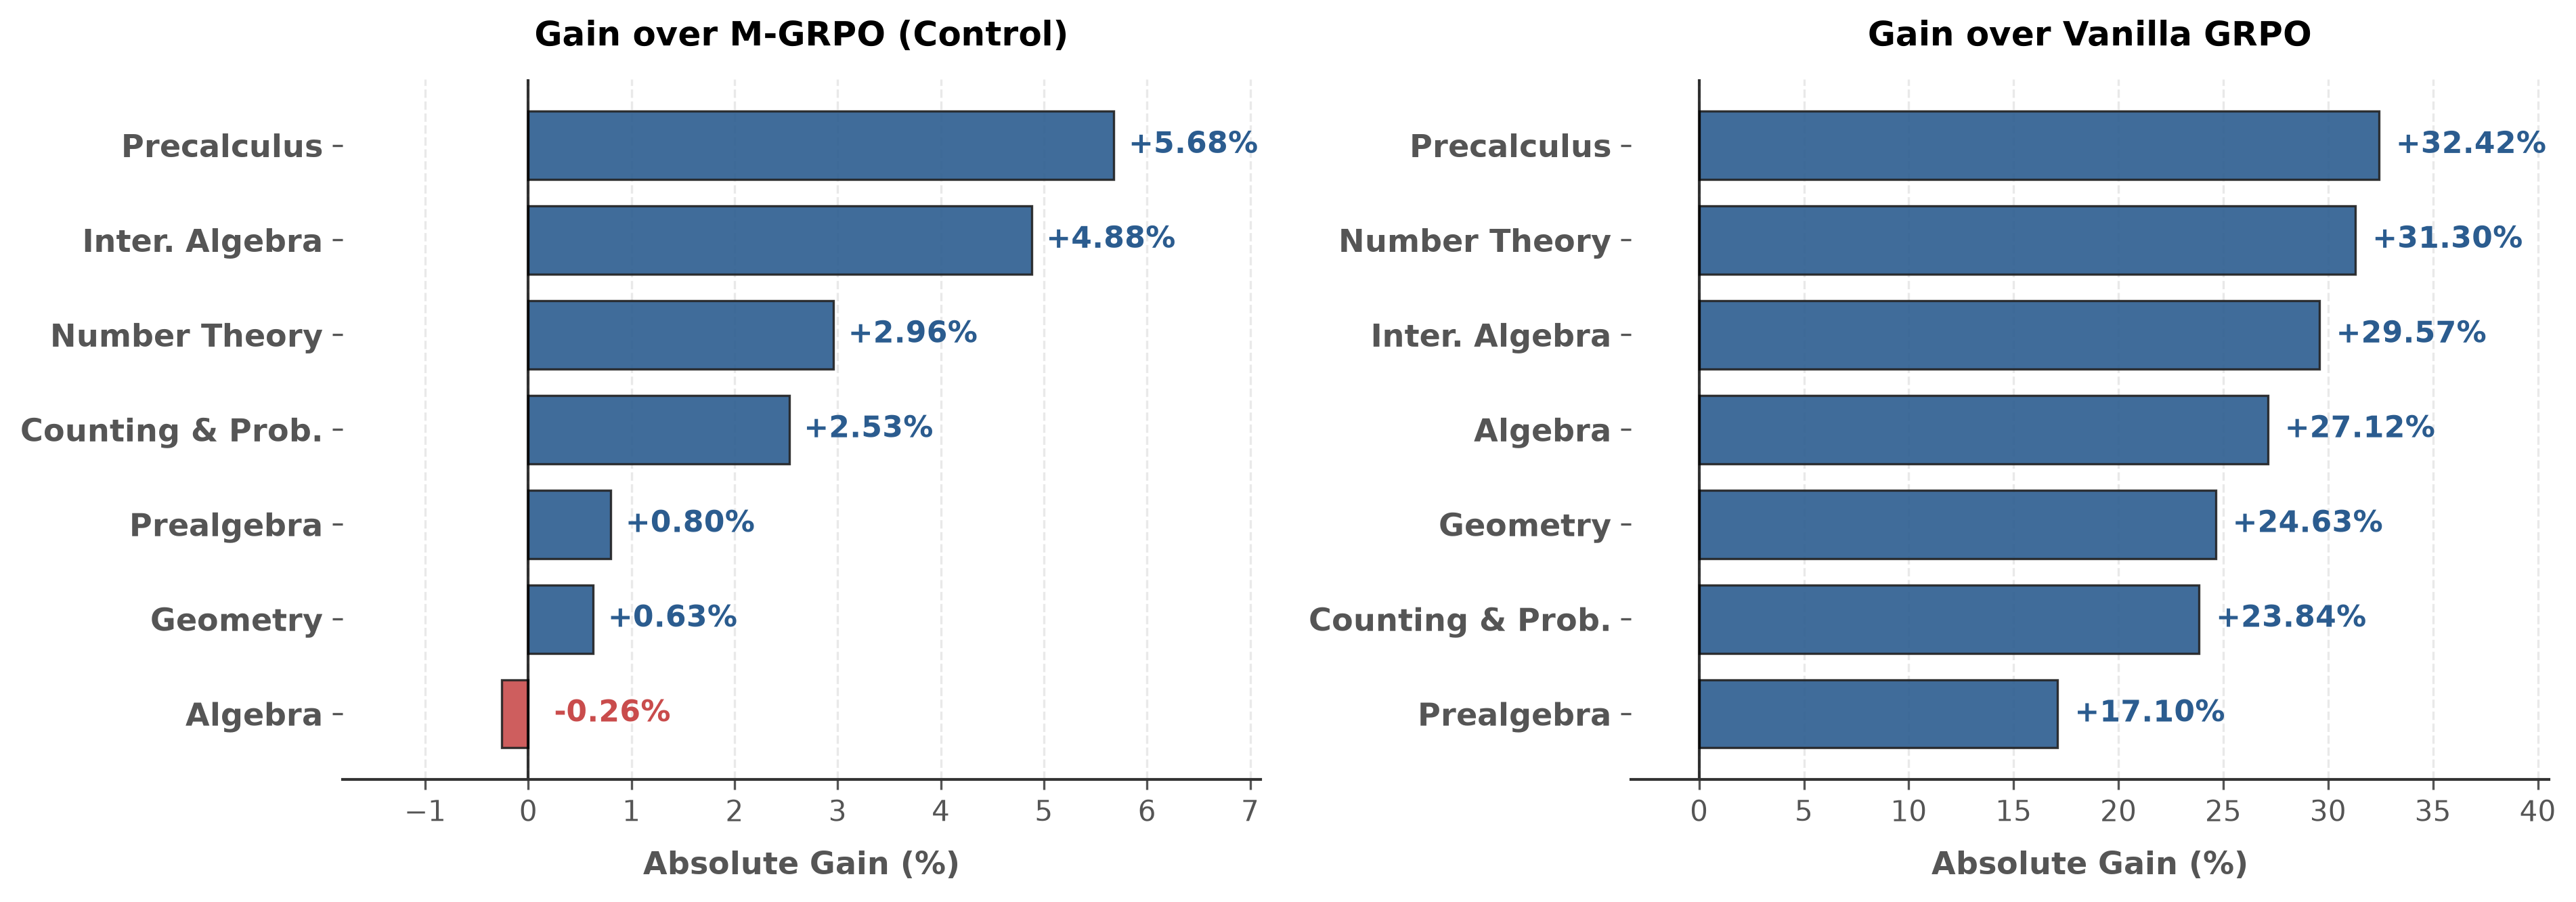
\includegraphics[width=0.76\textwidth]{math_delta_chart_combined.png}
\caption{Absolute performance gains of SB-GRPO on MATH sub-categories. \textbf{Top:} Compared to M-GRPO, showing pronounced improvements in \textit{Intermediate Algebra} (+4.88\%) and \textit{Precalculus} (+5.68\%). \textbf{Bottom:} Compared to Vanilla GRPO, highlighting broad gains achieved by multi-layer reasoning.}
\label{fig:delta}
\end{figure}

\subsection{Analysis}
The results demonstrate that SB-GRPO's core strength lies in resolving high-complexity reasoning tasks:

\textbf{Single-Sample Evaluation (Table \ref{tab:main}):} Under 1-sample greedy decoding, SB-GRPO achieves +2.20\% on MATH-500, +3.33\% on AIME 2024, and +1.01\% on GPQA Diamond over M-GRPO. On AIME 2025, SB-GRPO achieves 6.67\%, performing on par with M-GRPO ($\Delta_{S-M} = 0.00\%$) in this single-sample snapshot. Because AIME comprises only 30 problems, single-pass evaluations exhibit discrete quantization granularity ($\pm 3.33\%$ per problem), where a difference of a single question dictates the metric. This directly motivated our multi-pass evaluation protocol to capture true generative consistency.

\textbf{Multi-Sample Evaluation (Table \ref{tab:pass4}):} Across multi-sample generation (4 passes per problem) with distinct seeds on the trained policy, the advantages of semantic balancing become statistically robust. Table \ref{tab:pass4} reports Pass@1 accuracy alongside standard errors ($\text{mean} \pm \text{stderr}$) directly computed by the \texttt{lighteval} evaluation framework. SB-GRPO achieves $75.65 \pm 1.65\%$ on MATH-500 (+3.35\% over M-GRPO) and $33.08 \pm 2.45\%$ on GPQA Diamond (+3.66\%). Crucially, on AIME 2025, multi-pass evaluation breaks the single-sample tie, with SB-GRPO achieving $8.33 \pm 3.46\%$ (10/120 solved) vs. $6.67 \pm 3.38\%$ (8/120 solved) for M-GRPO. On AIME 2024, SB-GRPO achieves $12.50 \pm 4.91\%$ (15/120) compared to $10.83 \pm 4.59\%$ (13/120) for M-GRPO and $1.67 \pm 1.67\%$ (2/120) for Vanilla GRPO. This multi-sample protocol confirms that gains are consistent across diverse generation seeds rather than stochastic single-pass anomalies.

\textbf{Sub-category Analysis (Table \ref{tab:math}):} As depicted in Fig. \ref{fig:delta}, SB-GRPO exhibits its most substantial advantages in rigorous multi-stage disciplines: Precalculus (+5.68\%) and Intermediate Algebra (+4.88\%). For saturated domains like elementary Algebra ($\sim 89\%$ accuracy), failure modes are predominantly sporadic arithmetic slips rather than structural logical flaws; the entropy loss scaling factor adaptively downscales updates to preserve policy representations, yielding performance parity (89.13\% vs 89.39\%, -0.26\%).

\subsection{Ablation Analysis: Deconstructing the Performance Gains}
To understand how individual components contribute to the final gains, we systematically deconstruct the three core mechanisms of SB-GRPO and examine their operational effects:

\textbf{1. Role of Heuristic Confidence Gate ($\Gamma$) and Advantage Calibration:} In standard GRPO, whenever a rollout group is uniform ($R=0$ or $R=1$), reward variance vanishes ($\sigma \to 0$), reducing advantage values to zero ($A_{\text{std}}=0$) and stalling policy gradients entirely (Case 1, Sec.~\ref{subsec:heuristic_gate}). Ablating $\Gamma$ leads to repeated zero-gradient updates on difficult prompts. The gate smoothly activates virtual-reward calibration ($A_{\text{calib}}$) for uniform batches, sustaining continuous gradient flow without inducing optimization spikes.

\textbf{2. Role of Semantic Error Profiling (SEP) and Static Balanced Batching:} M-GRPO represents the structural ablation where two-layer reflection is enabled, but revisions are sampled uniformly without semantic clustering or balance. As shown in Table \ref{tab:main}, naive reflection plateaus at 72.60\% on MATH-500. Replacing uniform sampling with SEP and static 50/50 balanced batches ($S=16$) concentrates gradient descent on the dominant error cluster ($C_{\text{top}}$) while maintaining parity with verified reasoning paths, delivering an immediate +2.20\% gain.

\textbf{3. Role of Information-Theoretic Loss Scaling ($\lambda$):} Without entropy loss scaling ($\lambda = 1.0$), the policy treats all errors with equal update magnitude. The GSM8K results (Sec.~\ref{subsec:discussion}) illustrate why this is sub-optimal: simple arithmetic slips produce high semantic entropy across clusters, where $\lambda = \exp(-H/\tau)$ adaptively attenuates updates to prevent overfitting to superficial noise. When errors concentrate into a systematic fallacy (low $H$), $\lambda$ scales up to enforce decisive error unlearning.

\textbf{4. Structural Mitigation of Correction Bias in Self-Reflection:} A primary motivation of SB-GRPO is counteracting the \textit{Compulsive Correction Fallacy} inherent to unguided multi-layer reflection. In standard reflective GRPO (M-GRPO), prompting reflection unconditionally often induces models to second-guess valid intermediate deductions, converting initially correct solutions into incorrect revisions (false-negative drift). SB-GRPO structurally counters this vulnerability through two design choices: (i) an objective, neutral reflection prompt (Sec.~\ref{subsec:layer-generation-reflection}) that prevents biasing the policy toward unwarranted modifications, and (ii) Static Balanced Batching ($S/2$ verified trajectories paired with $S/2$ from $C_{\text{top}}$), preventing gradient updates from being skewed by negative paths. This architectural pairing stabilizes correct reasoning paths while strictly targeting persistent, clustered logical flaws.

\subsection{Discussion}\label{subsec:discussion}
\textbf{The GSM8K Trade-Off:} SB-GRPO scores 69.22\% on GSM8K compared to M-GRPO's 70.51\%. GSM8K consists primarily of elementary word problems with short reasoning chains, where incorrect answers stem from stochastic calculation slips rather than structural logical flaws. Consequently, semantic entropy $H$ remains uniformly high, prompting $\lambda$ to dampen gradient updates. While M-GRPO overfits to these arithmetic noise samples, SB-GRPO preserves representational stability, translating into decisive superiority on advanced benchmarks.

\textbf{Qualitative Inspection of Semantic Error Clusters:} Qualitative inspection of the Top Error Cluster ($C_{\text{top}}$) confirms our core premise: on Intermediate Algebra and Precalculus problems in MATH-500, incorrect rollouts within $C_{\text{top}}$ consistently share identical mathematical misconceptions---such as misapplying sign reversals in quadratic inequalities or neglecting boundary conditions in logarithmic domains---rather than arbitrary lexical overlap. This demonstrates that frozen MiniLM embeddings reliably isolate systematic logical flaws.